\documentclass[border=7pt]{standalone}
\usepackage{mathptmx}
\usepackage{tikz}
\usetikzlibrary{arrows.meta,shadows}

\definecolor{ink}{HTML}{3A3936}
\definecolor{muted}{HTML}{656461}
\definecolor{dataF}{HTML}{F0EFEC}
\definecolor{modelE}{HTML}{2A78D6}\definecolor{modelF}{HTML}{DCE9F9}
\definecolor{augE}{HTML}{EB6834}\definecolor{augF}{HTML}{FDE3D6}
\definecolor{opE}{HTML}{6250D6}\definecolor{opF}{HTML}{EBE9FB}
\definecolor{lossE}{HTML}{1BAF7A}\definecolor{lossF}{HTML}{D9F3E9}

\tikzset{
  every node/.style={font=\small,text=ink,align=center},
  base/.style={rectangle,rounded corners=3pt,minimum height=12mm,inner sep=3pt,line width=0.8pt},
  data/.style={base,fill=dataF,draw=muted,text width=23mm},
  model/.style={base,fill=modelF,draw=modelE,text width=25mm},
  aug/.style={base,fill=augF,draw=augE,line width=1.2pt,text width=24mm},
  target/.style={base,fill=opF,draw=opE,text width=42mm},
  loss/.style={base,fill=lossF,draw=lossE,text width=30mm},
  tensor/.style={rectangle,fill=white,draw=modelE,line width=.8pt,minimum width=7mm,minimum height=9mm,
    double copy shadow={shadow xshift=1.5pt,shadow yshift=1.5pt,draw=modelE,fill=white}},
  flow/.style={-{Stealth[length=2.3mm]},line width=.8pt,draw=ink,rounded corners=4pt},
  fixed/.style={flow,densely dashed,draw=opE},
  note/.style={font=\footnotesize\itshape,text=muted},
}
\newcommand{\sub}{\footnotesize\color{muted}}


\begin{document}
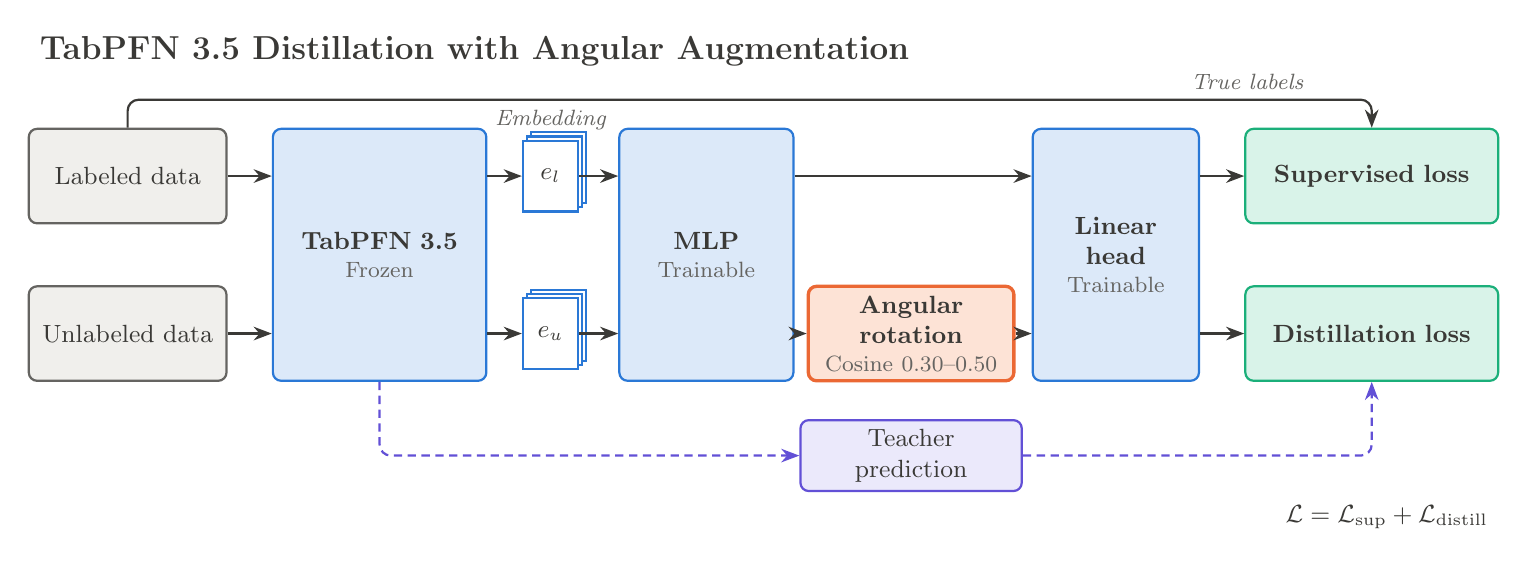
\begin{tikzpicture}
\node[anchor=west,font=\large\bfseries] at (-1.24,1.58) {TabPFN 3.5 Distillation with Angular Augmentation};

\node[data] (xl) at (0,0) {Labeled data};
\node[data] (xu) at (0,-2) {Unlabeled data};
\node[model,minimum height=32mm] (tabpfn) at (3.2,-1) {\textbf{TabPFN 3.5}\\[-1pt]{\sub Frozen}};
\node[tensor] (el) at (5.37,0) {$e_l$};
\node[tensor] (eu) at (5.37,-2) {$e_u$};
\node[note,above] at (el.north) {Embedding};
\node[model,text width=20mm,minimum height=32mm] (mlp) at (7.35,-1) {\textbf{MLP}\\[-1pt]{\sub Trainable}};
\node[aug] (aug) at (9.95,-2) {\textbf{Angular rotation}\\[-1pt]{\sub Cosine 0.30--0.50}};
\node[model,text width=19mm,minimum height=32mm] (head) at (12.55,-1) {\textbf{Linear head}\\[-1pt]{\sub Trainable}};
\node[loss] (sup) at (15.8,0) {\textbf{Supervised loss}};
\node[loss] (dist) at (15.8,-2) {\textbf{Distillation loss}};
\node[target,text width=26mm,minimum height=9mm] (teacher) at (9.95,-3.55) {Teacher prediction};

\draw[flow] (xl.east) -- (xl -| tabpfn.west);
\draw[flow] (xu.east) -- (xu -| tabpfn.west);
\draw[flow] (tabpfn.east |- el) -- (el.west);
\draw[flow] (tabpfn.east |- eu) -- (eu.west);
\draw[flow] (el.east) -- (el -| mlp.west);
\draw[flow] (eu.east) -- (eu -| mlp.west);
\draw[flow] (mlp.east |- el) -- (el -| head.west);
\draw[flow] (mlp.east |- aug) -- (aug.west);
\draw[flow] (aug.east) -- (aug -| head.west);
\draw[flow] (head.east |- sup) -- (sup.west);
\draw[flow] (head.east |- dist) -- (dist.west);
\draw[flow] (xl.north) -- (0,.97) -- node[note,above,pos=.9] {True labels} (15.8,.97) -- (sup.north);
\draw[fixed] (tabpfn.south) |- (teacher.west);
\draw[fixed] (teacher.east) -| (dist.south);

\node[anchor=east] at (17.4,-4.33) {$\mathcal L = \mathcal L_{\mathrm{sup}} + \mathcal L_{\mathrm{distill}}$};
\end{tikzpicture}
\end{document}
